\documentclass[parskip=half]{scrartcl}

\usepackage[T1]{fontenc}
\usepackage[utf8]{inputenc}
\usepackage{amsmath, amsfonts}
\usepackage{tikz}
\usepackage{hyperref}

\title{Migros Cross-Math Solver}
\author{Pascal Lüscher}

\newcommand{\rect}[4]{\draw[fill=#4] (#1 cm, #2 cm) rectangle (#1 cm + 1 cm, #2 cm - 1 cm) node[pos=.5] {#3};}


\newcommand{\wsq}[3]{\rect{#1}{#2}{#3}{white}}
\newcommand{\bsq}[2]{\rect{#1}{#2}{}{gray}}
\newcommand{\ysq}[2]{\rect{#1}{#2}{}{yellow!10}}
\newcommand{\solCell}[3]{\rect{#1}{#2}{#3}{yellow!5}}

\newcommand{\onetonine}{\{1,\ldots,9\}}


\begin{document}

\maketitle

\section{Problem}
The Cross-Math puzzle is a puzzle with 9 numbers to fill.
The rules are simple:
\begin{itemize}
	\item Mathematical operation ordering does not count, simply calc from left to right and from top to bottom
	\item Each cell is filled with a number between 1 - 9
	\item Each number can only appear once
\end{itemize}

The puzzle presented is the following:
\begin{center}
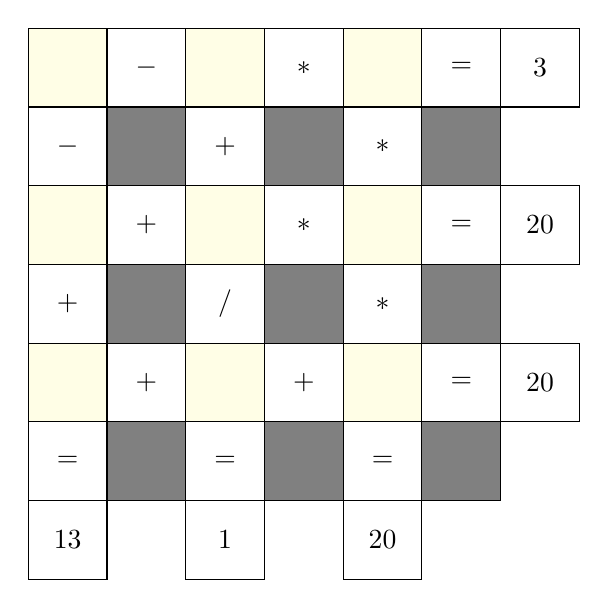
\begin{tikzpicture}
	\ysq{0}{7};
	\wsq{1}{7}{$-$};
	\ysq{2}{7};
	\wsq{3}{7}{$*$};
	\ysq{4}{7};
	\wsq{5}{7}{$=$};
	\wsq{6}{7}{$3$};

	\wsq{0}{6}{$-$}
	\bsq{1}{6}
	\wsq{2}{6}{$+$}
	\bsq{3}{6}
	\wsq{4}{6}{$*$}
	\bsq{5}{6}
	
	\ysq{0}{5};
	\wsq{1}{5}{$+$};
	\ysq{2}{5};
	\wsq{3}{5}{$*$};
	\ysq{4}{5};
	\wsq{5}{5}{$=$};
	\wsq{6}{5}{$20$};
	
	\wsq{0}{4}{$+$}
	\bsq{1}{4}
	\wsq{2}{4}{$/$}
	\bsq{3}{4}
	\wsq{4}{4}{$*$}
	\bsq{5}{4}
	
	\ysq{0}{3};
	\wsq{1}{3}{$+$};
	\ysq{2}{3};
	\wsq{3}{3}{$+$};
	\ysq{4}{3};
	\wsq{5}{3}{$=$};
	\wsq{6}{3}{$20$};
	
	\wsq{0}{2}{$=$}
	\bsq{1}{2}
	\wsq{2}{2}{$=$}
	\bsq{3}{2}
	\wsq{4}{2}{$=$}
	\bsq{5}{2}

	\wsq{0}{1}{$13$}
	\wsq{2}{1}{$1$}
	\wsq{4}{1}{$20$}
\end{tikzpicture}
\end{center}


\section{Mathematical formulation}
\subsection{With Big-$M$}

\begin{align}
&\min \quad &&0 \\
& \text{s.t.} \quad 
  && x_i 			&&\geq 1 		,&&\quad \forall i \in \onetonine \label{eq:basicmin1} \\
& && x_i 			&&\leq 9  		,&&\quad \forall i \in \onetonine \label{eq:basicmax9} \\
& && x_i - x_j 	&&\leq -\epsilon + y_{i,j} M ,&& \quad \forall i,j \in \onetonine \label{eq:basicm1}\\
& && x_i - x_j 	&&\geq \epsilon - (1-y_{i,j}) M ,&& \quad \forall i,j \in \onetonine \label{eq:basicm2}\\
& && (x_0 - x_1) x_2  &&= 3 \label{eq:problemh1} \\
& && (x_3 + x_4) x_5  &&= 20 \label{eq:problemh2} \\
& && x_6  + x_7 + x_8 &&= 20 \label{eq:problemh3} \\
& && x_0 - x_3 + x_6  &&= 13 \label{eq:problemv1} \\
& && \frac{(x_1 + x_4)}{x_7} ,&&= 1 \label{eq:problemv2} \\
& && x_2  x_5  x_8 &&= 20 \label{eq:problemv3} \\
& && x_i 		&&\in \mathbb{N}  ,&& \quad \forall i \in \onetonine \\
& && y_{i,j} 		&&\in \{0,1\} ,&& \quad \forall i,j \in \onetonine \\
\end{align}
$M$ is very big and $\epsilon$ is a very small number.

\autoref{eq:basicmin1} -- \autoref{eq:basicm2} are the basic requirements for the corss-math puzzle. \autoref{eq:problemh1} -- \autoref{eq:problemv3} are the specific equations for this problem.
\pagebreak
\subsection{One Hot Matrix}

The idea behind a one hot matrix is to add a binary variable for each possibility. In our case this means to add 9 binary variables for every field.


\begin{align}
&\min \quad &&0 \\
& \text{s.t.} \quad 
&& \sum_{j=1}^{j\leq 9}x_{i,j}   &&= 1 		,&&\quad \forall i \in \onetonine \label{eq:basics1} \\
& && \sum_{i=1}^{i\leq 9}x_{i,j} 			&&=1  		,&&\quad \forall j \in \onetonine \label{eq:basics2} \\
& && y_i &&= \sum_{j=1}^{j\leq 9} jx_{i,j}  ,&&\quad \forall i \in \onetonine \label{eq:vali} \\
& && (y_0 - y_1) y_2  &&= 3 \label{eq:2problemh1} \\
& && (y_3 + y_4) y_5  &&= 20 \label{eq:2problemh2} \\
& && y_6  + y_7 + y_8 &&= 20 \label{eq:2problemh3} \\
& && y_0 - y_3 + y_6  &&= 13 \label{eq:2problemv1} \\
& && \frac{(y_1 + y_4)}{y_7} &&= 1 \label{eq:2problemv2} \\
& && y_2  y_5  y_8 &&= 20 \label{eq:2problemv3} \\
& && x_{i,j} 		&&\in \{0,1\} ,&& \quad \forall i,j \in \onetonine \\
\end{align}

The constraints \autoref{eq:basics1} and \autoref{eq:basics2} define the uniqueness of a number in the problem. With \autoref{eq:vali} a linear expression $y_i$ is defined that expresses the actual value of the cell $i$. This linear expression is then used in \autoref{eq:2problemh1} -- \autoref{eq:2problemv3} to define the actual problem. These constraints are the same as \autoref{eq:problemh1} -- \autoref{eq:problemv3}.

\section{Solution}
\begin{center}
	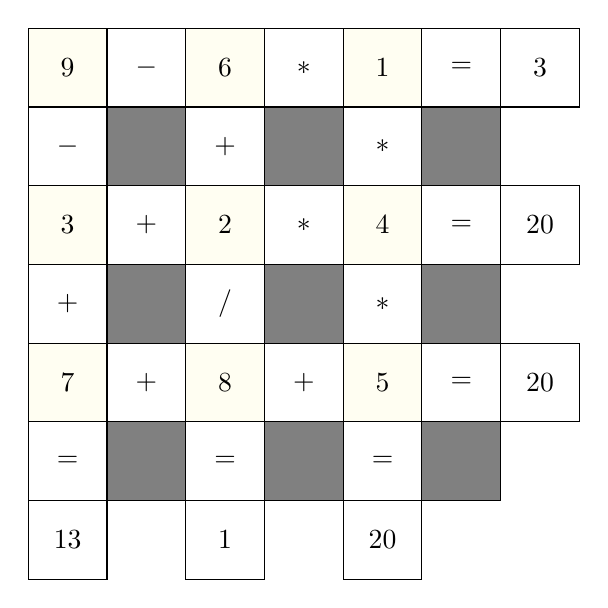
\begin{tikzpicture}
		\solCell{0}{7}{$9$};
		\wsq{1}{7}{$-$};
		\solCell{2}{7}{$6$};
		\wsq{3}{7}{$*$};
		\solCell{4}{7}{$1$};
		\wsq{5}{7}{$=$};
		\wsq{6}{7}{$3$};
		
		\wsq{0}{6}{$-$}
		\bsq{1}{6}
		\wsq{2}{6}{$+$}
		\bsq{3}{6}
		\wsq{4}{6}{$*$}
		\bsq{5}{6}
		
		\solCell{0}{5}{$3$};
		\wsq{1}{5}{$+$};
		\solCell{2}{5}{$2$};
		\wsq{3}{5}{$*$};
		\solCell{4}{5}{$4$};
		\wsq{5}{5}{$=$};
		\wsq{6}{5}{$20$};
		
		\wsq{0}{4}{$+$}
		\bsq{1}{4}
		\wsq{2}{4}{$/$}
		\bsq{3}{4}
		\wsq{4}{4}{$*$}
		\bsq{5}{4}
		
		\solCell{0}{3}{$7$};
		\wsq{1}{3}{$+$};
		\solCell{2}{3}{$8$};
		\wsq{3}{3}{$+$};
		\solCell{4}{3}{$5$};
		\wsq{5}{3}{$=$};
		\wsq{6}{3}{$20$};
		
		\wsq{0}{2}{$=$}
		\bsq{1}{2}
		\wsq{2}{2}{$=$}
		\bsq{3}{2}
		\wsq{4}{2}{$=$}
		\bsq{5}{2}
		
		\wsq{0}{1}{$13$}
		\wsq{2}{1}{$1$}
		\wsq{4}{1}{$20$}
	\end{tikzpicture}
\end{center}
\end{document}
